
%(BEGIN_QUESTION)
% Copyright 2015, Tony R. Kuphaldt, released under the Creative Commons Attribution License (v 1.0)
% This means you may do almost anything with this work of mine, so long as you give me proper credit

A helpful strategy for qualitatively analyzing control strategies is to mark the inputs of multi-input functions shown in those strategies with either ``+'' or ``$-$'' labels to denote direction of action.  This is the same symbology used to mark the inputs of an operational amplifier, where ``+'' represents the noninverting input and ``$-$'' represents the inverting input.  In fact, one might think of an operational amplifier as being a proportional controller with a really large gain ($k$) value:

$$\includegraphics[width=15.5cm]{i01171x01.eps}$$

To illustrate this concept, examine these two diagrams of a single-loop control system.  In the left-hand diagram, the controller is shown using standard ISA symbology.  In the right-hand sketch, the controller is shown using opamp symbology instead.  In both cases, the controller must be {\it reverse-acting} in order to stabilize the process, but the ``+'' and ``$-$'' symbols make it easier to distinguish the directions of action for the process variable versus the setpoint:

$$\includegraphics[width=15.5cm]{i01171x02.eps}$$

\filbreak

Sketch your own ``+'' and ``$-$'' labels at the input(s) of each controller in each of these control strategy diagrams, to denote the proper directions of action to make each system work properly.  In order to help you do this, the right-hand version of each diagram uses opamp symbology for the controller rather than ISA symbology.  Assume the use of direct-acting transmitters in each case, and be sure to pay close attention to each control valve's direction of action:

$$\includegraphics[width=15.5cm]{i01171x03.eps}$$

\vskip 20pt \vbox{\hrule \hbox{\strut \vrule{} {\bf Suggestions for Socratic discussion} \vrule} \hrule}

\begin{itemize}
\item{} Perform a series of ``thought experiments'' where you imagine the process variable changing value due to some change in process load, and then analyze the action taken by each controller in each control system.  How do the ``+'' and ``$-$'' labels aid your analysis of each system?
\item{} What do you notice about the respective actions of the master and slave controllers in the cascade systems, and how those actions must be for ATO versus ATC valves?  Does this result surprise you at all?
\item{} Explain why it only makes sense to label the {\it inputs} of a controller with ``polarity'' symbols and not the {\it output} of a controller.
\end{itemize}

\underbar{file i01171}
%(END_QUESTION)





%(BEGIN_ANSWER)

$$\includegraphics[width=15.5cm]{i01171x04.eps}$$

Note that the words ``direct'' and ``reverse'' are redundant to the ``+'' and ``$-$'' labels.  A controller with a ``+'' label at its PV input is by definition direct-acting; a controller with a ``$-$'' label at its PV input is by definition reverse-acting.
 
%(END_ANSWER)





%(BEGIN_NOTES)

Here are the necessary controller actions shown if the control valve is Air-To-Close (ATC) instead of Air-To-Open (ATO):

$$\includegraphics[width=15.5cm]{i01171x05.eps}$$


%INDEX% Basics, control: direct versus reverse controller action
%INDEX% Control, strategies: cascaded controller action

%(END_NOTES)


